\documentclass[tikz,border=4pt]{standalone}
% Shared style for MultiMM figures (white background, logo palette)
\usepackage{tikz,pgfplots,amsmath}
\pgfplotsset{compat=1.16}
\usetikzlibrary{arrows.meta,calc,decorations.pathreplacing,positioning,backgrounds}
\definecolor{indigo}{HTML}{3B37A0}
\definecolor{violet}{HTML}{6A3AA8}
\definecolor{crimson}{HTML}{B5406C}
\definecolor{gold}{HTML}{E9A62C}
\definecolor{golddark}{HTML}{B9791A}
\definecolor{grey}{HTML}{8A8AA0}
\definecolor{lightgrey}{HTML}{E4E4EE}
\tikzset{
  bead/.style={circle,draw=#1!80!black,fill=#1!35,line width=0.5pt,minimum size=9pt,inner sep=0pt},
  bead/.default=indigo,
  lab/.style={font=\small},
}
\pgfplotsset{
  every axis/.append style={
    width=9.5cm,height=6.3cm,axis lines=left,line width=0.5pt,
    grid=major,grid style={draw=lightgrey,line width=0.3pt},
    tick label style={font=\small},label style={font=\normalsize},
    legend style={font=\footnotesize,draw=none,fill=white,fill opacity=0.8,text opacity=1},
    legend cell align=left,
  },
  every axis plot/.append style={line width=1.2pt,smooth},
}

\begin{document}
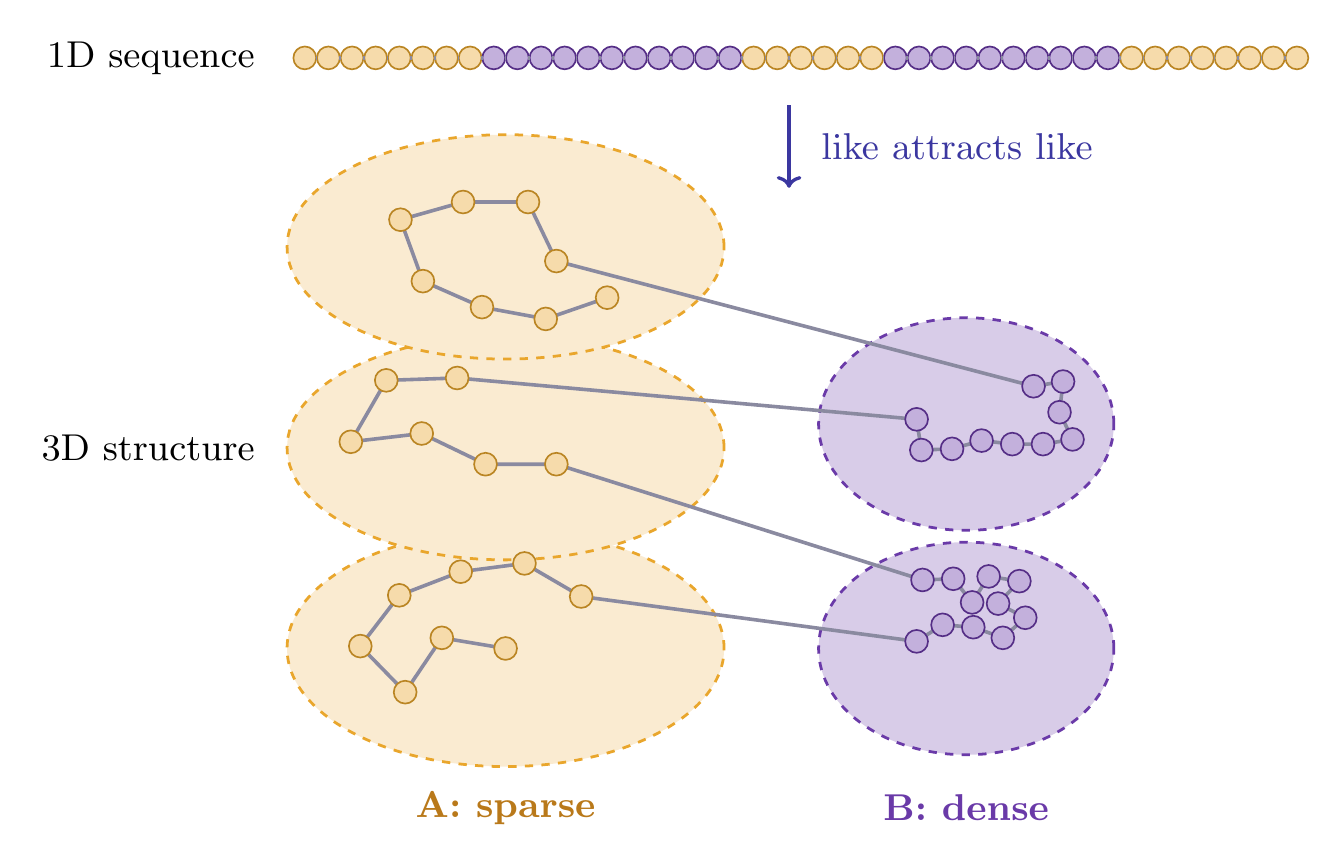
\begin{tikzpicture}[scale=1.5,every node/.append style={transform shape}]
\tikzset{sb/.style={circle,draw=#1!80!black,fill=#1!40,line width=0.6pt,minimum size=5.5pt,inner sep=0pt}}
\node[sb=gold] (s0) at (0.00,0) {};
\node[sb=gold] (s1) at (0.20,0) {};
\node[sb=gold] (s2) at (0.40,0) {};
\node[sb=gold] (s3) at (0.60,0) {};
\node[sb=gold] (s4) at (0.80,0) {};
\node[sb=gold] (s5) at (1.00,0) {};
\node[sb=gold] (s6) at (1.20,0) {};
\node[sb=gold] (s7) at (1.40,0) {};
\node[sb=violet] (s8) at (1.60,0) {};
\node[sb=violet] (s9) at (1.80,0) {};
\node[sb=violet] (s10) at (2.00,0) {};
\node[sb=violet] (s11) at (2.20,0) {};
\node[sb=violet] (s12) at (2.40,0) {};
\node[sb=violet] (s13) at (2.60,0) {};
\node[sb=violet] (s14) at (2.80,0) {};
\node[sb=violet] (s15) at (3.00,0) {};
\node[sb=violet] (s16) at (3.20,0) {};
\node[sb=violet] (s17) at (3.40,0) {};
\node[sb=violet] (s18) at (3.60,0) {};
\node[sb=gold] (s19) at (3.80,0) {};
\node[sb=gold] (s20) at (4.00,0) {};
\node[sb=gold] (s21) at (4.20,0) {};
\node[sb=gold] (s22) at (4.40,0) {};
\node[sb=gold] (s23) at (4.60,0) {};
\node[sb=gold] (s24) at (4.80,0) {};
\node[sb=violet] (s25) at (5.00,0) {};
\node[sb=violet] (s26) at (5.20,0) {};
\node[sb=violet] (s27) at (5.40,0) {};
\node[sb=violet] (s28) at (5.60,0) {};
\node[sb=violet] (s29) at (5.80,0) {};
\node[sb=violet] (s30) at (6.00,0) {};
\node[sb=violet] (s31) at (6.20,0) {};
\node[sb=violet] (s32) at (6.40,0) {};
\node[sb=violet] (s33) at (6.60,0) {};
\node[sb=violet] (s34) at (6.80,0) {};
\node[sb=gold] (s35) at (7.00,0) {};
\node[sb=gold] (s36) at (7.20,0) {};
\node[sb=gold] (s37) at (7.40,0) {};
\node[sb=gold] (s38) at (7.60,0) {};
\node[sb=gold] (s39) at (7.80,0) {};
\node[sb=gold] (s40) at (8.00,0) {};
\node[sb=gold] (s41) at (8.20,0) {};
\node[sb=gold] (s42) at (8.40,0) {};
\foreach \i in {0,...,41}{\pgfmathtruncatemacro{\j}{\i+1}\draw[grey,line width=1.3pt] (s\i)--(s\j);}
\node[lab,anchor=east] at (-0.3,0) {1D sequence};
\draw[->,line width=1.2pt,indigo] (4.1,-0.4)--(4.1,-1.1);
\node[lab,indigo,anchor=west] at (4.25,-0.75) {like attracts like};
\begin{scope}[shift={(0,-5.0)}]
\node[lab,anchor=east] at (-0.3,1.7) {3D structure};
\fill[gold!22,draw=gold,line width=1pt,dashed] (1.7,0.0) ellipse (1.85 and 1.0);
\fill[violet!26,draw=violet,line width=1pt,dashed] (5.6,0.0) ellipse (1.25 and 0.8999999999999999);
\fill[gold!22,draw=gold,line width=1pt,dashed] (1.7,1.7) ellipse (1.85 and 0.95);
\fill[violet!26,draw=violet,line width=1pt,dashed] (5.6,1.9) ellipse (1.25 and 0.8999999999999999);
\fill[gold!22,draw=gold,line width=1pt,dashed] (1.7,3.4) ellipse (1.85 and 0.95);
\draw[grey,line width=1.3pt] (1.70,0.00) -- (1.16,0.09) -- (0.85,-0.37) -- (0.47,0.02) -- (0.80,0.45) -- (1.32,0.65) -- (1.86,0.72) -- (2.34,0.44) -- (5.18,0.06) -- (5.40,0.20) -- (5.66,0.18) -- (5.91,0.09) -- (6.10,0.26) -- (5.87,0.38) -- (6.05,0.57) -- (5.79,0.61) -- (5.65,0.39) -- (5.49,0.59) -- (5.23,0.58) -- (2.13,1.56) -- (1.53,1.56) -- (0.99,1.82) -- (0.39,1.75) -- (0.69,2.27) -- (1.29,2.29) -- (5.18,1.94) -- (5.22,1.68) -- (5.48,1.69) -- (5.73,1.76) -- (5.99,1.73) -- (6.25,1.73) -- (6.50,1.77) -- (6.39,2.00) -- (6.42,2.26) -- (6.17,2.22) -- (2.13,3.28) -- (1.89,3.78) -- (1.34,3.78) -- (0.81,3.63) -- (1.00,3.11) -- (1.50,2.89) -- (2.04,2.79) -- (2.56,2.97);
\node[sb=gold] at (1.70,0.00) {};
\node[sb=gold] at (1.16,0.09) {};
\node[sb=gold] at (0.85,-0.37) {};
\node[sb=gold] at (0.47,0.02) {};
\node[sb=gold] at (0.80,0.45) {};
\node[sb=gold] at (1.32,0.65) {};
\node[sb=gold] at (1.86,0.72) {};
\node[sb=gold] at (2.34,0.44) {};
\node[sb=violet] at (5.18,0.06) {};
\node[sb=violet] at (5.40,0.20) {};
\node[sb=violet] at (5.66,0.18) {};
\node[sb=violet] at (5.91,0.09) {};
\node[sb=violet] at (6.10,0.26) {};
\node[sb=violet] at (5.87,0.38) {};
\node[sb=violet] at (6.05,0.57) {};
\node[sb=violet] at (5.79,0.61) {};
\node[sb=violet] at (5.65,0.39) {};
\node[sb=violet] at (5.49,0.59) {};
\node[sb=violet] at (5.23,0.58) {};
\node[sb=gold] at (2.13,1.56) {};
\node[sb=gold] at (1.53,1.56) {};
\node[sb=gold] at (0.99,1.82) {};
\node[sb=gold] at (0.39,1.75) {};
\node[sb=gold] at (0.69,2.27) {};
\node[sb=gold] at (1.29,2.29) {};
\node[sb=violet] at (5.18,1.94) {};
\node[sb=violet] at (5.22,1.68) {};
\node[sb=violet] at (5.48,1.69) {};
\node[sb=violet] at (5.73,1.76) {};
\node[sb=violet] at (5.99,1.73) {};
\node[sb=violet] at (6.25,1.73) {};
\node[sb=violet] at (6.50,1.77) {};
\node[sb=violet] at (6.39,2.00) {};
\node[sb=violet] at (6.42,2.26) {};
\node[sb=violet] at (6.17,2.22) {};
\node[sb=gold] at (2.13,3.28) {};
\node[sb=gold] at (1.89,3.78) {};
\node[sb=gold] at (1.34,3.78) {};
\node[sb=gold] at (0.81,3.63) {};
\node[sb=gold] at (1.00,3.11) {};
\node[sb=gold] at (1.50,2.89) {};
\node[sb=gold] at (2.04,2.79) {};
\node[sb=gold] at (2.56,2.97) {};
\node[lab,golddark,font=\bfseries\small] at (1.7,-1.35) {A: sparse};
\node[lab,violet,font=\bfseries\small] at (5.6,-1.35) {B: dense};
\end{scope}
\end{tikzpicture}
\end{document}
